\documentclass[a4paper,12pt]{article}
\usepackage[english,russian]{babel}
\usepackage{fontspec}
\defaultfontfeatures{Ligatures={TeX},Renderer=Basic}
\setmainfont[Ligatures={TeX,Historic}]{Calibri Light}
\setsansfont{Calibri Light}
\setmonofont{Consolas}

\usepackage{indentfirst}
\frenchspacing

% Для математики
\usepackage{amssymb,amsmath}
\setcounter{MaxMatrixCols}{20}
\parindent=24pt
\parskip=0pt
\tolerance=2000

% Для настройки размера страницы
\usepackage{geometry}
\geometry{
	a4paper,
	total={170mm,257mm},
	left=20mm,
	top=20mm,
}

% Для вставки графики
\usepackage{graphicx}

% Для таблиц
\usepackage{longtable}
\usepackage{multirow}
\usepackage{tabu}
\usepackage{colortbl}
\usepackage{hhline}

% Создаем команду, чтобы переносить текст на новую строку внутри таблицы
\newcommand{\tcell}[2][c]{\begin{tabular}[#1]{@{}c@{}}#2\end{tabular}}

% Пакет для списков
\usepackage[ampersand]{easylist}

% Для контура вокруг текста
\usepackage[outline]{contour}

% Пакеты от tikz
\usepackage{tikz}
\usepackage{graphics}
\usepackage{pgfplots}
\usepackage{pgfplotstable}
\usepackage{xcolor}
\usetikzlibrary{calc}
\usetikzlibrary{through}
\usetikzlibrary{intersections}
\usetikzlibrary{patterns}
\usetikzlibrary{scopes}
\usetikzlibrary{decorations.pathreplacing}
\usetikzlibrary{arrows.meta}

% Для цветных таблиц
\usepackage{multicol}
\usepackage{tcolorbox}
\tcbuselibrary{skins}
\tcbuselibrary{breakable}
\tcbuselibrary{minted}
\usemintedstyle{vs}

% Для подсветки кода
\usepackage{minted}

% Задаем цвет номеров строк подсветки кода
\renewcommand{\theFancyVerbLine}{\sffamily\textcolor[rgb]{1, 1, 1}{\fontsize{4}{4}\selectfont\arabic{FancyVerbLine}}}

% Определяем новую команду для красивой вставки кода в рамочке и с прочими прелестями
\newcommand{\mycodeinput}[3]{
\begin{tcolorbox}[
	colback=black!5!white,
	colframe=black!30!white,
	boxrule=0.5pt, 
	listing only,
	left=-0.5mm,
	leftrule=3.3mm,
	arc=2mm, outer arc=2mm,
	top=0pt,
	bottom=0pt,
	enhanced jigsaw,
	breakable,
	title={#3},
	coltitle=black, 
	fonttitle=\bfseries\ttfamily,
	break at=-\baselineskip/0pt/\textheight, % Магия для работы multicols
	attach boxed title to top center={yshift=-1mm,yshifttext=-1mm},
	boxed title style={
		enhanced,
		nobeforeafter,
		tcbox raise base,
		boxrule=0.4pt,
		top=0.5mm,
		bottom=0.5mm,
		right=0mm,
		left=4mm,
		arc=1pt,
		boxsep=2pt,
		before upper={\vphantom{dlg}},
		colframe=black!30!white,
		colback=black!10!white,
		overlay={
			\begin{tcbclipinterior}
			\fill[black!30!white]
				(frame.south west)
					rectangle node[text=white,font=\sffamily\bfseries\scriptsize,rotate=90] {FILE} 
				([xshift=4mm]frame.north west);
			\end{tcbclipinterior}
		}
	},
]
\inputminted[
	breaklines,
	breakanywhere=true,
	autogobble,
	linenos,
	numbersep=1mm,
	mathescape, 
	fontsize=\fontsize{4}{4}\selectfont, 
	tabsize=4
]{#1}{#2}
\end{tcolorbox}
}

% Определяем новую команду для вставки кода прямо в тексте
\newtcbox{\inlinecodetable}{on line,
arc=2pt,colback=gray!10!white,colframe=gray!50!black,
before upper={\rule[-3pt]{0pt}{10pt}},boxrule=0.5pt,
boxsep=0pt,left=2pt,right=2pt,top=2pt,bottom=0pt}
\newcommand{\mycodeinline}[2]{\inlinecodetable{\mintinline{#1}{#2}}}

% Определяем новую команду для создания титульного листа
\newcommand{\mytitlepage}[9]{
\begin{center}
\hfill \break
\Large{Министерство образования и науки Российской Федерации}\\
\hfill \break
\large{Федеральное государственное бюджетное образовательное учреждение высшего образования}\\ 
\normalsize{\textbf{«НОВОСИБИРСКИЙ ГОСУДАРСТВЕННЫЙ ТЕХНИЧЕСКИЙ УНИВЕРСИТЕТ»}}\\
\hfill \break

\includegraphics{nstu_logo.eps} \\
\hfill \break
\large{Кафедра #1}\\
\hfill \break
\large{Лабораторная работа №#2\\по дисциплине <<#3>>}\\
\hfill \break
\hfill \break
\Large{\textbf{#4}}\\
\hfill \break
\hfill \break 
\normalsize{\begin{tabular}{cllp{1.5cm}p{1.5cm}}
\multirow{5}{*}[0.75cm]{
\includegraphics[scale=0.5]{fami_logo.eps}}
& \textbf{Факультет:} & ПМИ & & \\[1.25ex]
& \textbf{Группа:} & #5 & & \\[1.25ex]
& \textbf{Студент:} & #6 & & \\[1.25ex]
& \textbf{Вариант:} & #7 & & \\[1.25ex]
& \textbf{Преподаватель:} & #8 & & \\[1.25ex]
\end{tabular}} \\
\hfill \break
\hfill \break
\hfill \break
\hfill \break
\hfill \break
\large{Новосибирск\\#9}
\end{center}
\thispagestyle{empty}
\newpage 
\setcounter{page}{1}
}

\begin{document}

\mytitlepage{прикладной математики}{2}{Численные методы}{Итерационные методы решения СЛАУ}{ПМ-63}{Шепрут И.И.}{11}{Задорожный А.Г.}{2018}

\section{Цель работы}

Разработать программы решения СЛАУ методами Якоби, Гаусса-Зейделя с хранением матрицы в диагональном формате. Исследовать сходимость методов для различных тестовых матриц и её зависимость от параметра релаксации. Изучить возможность оценки порядка числа обусловленности матрицы путем вычислительного эксперимента.

\textbf{Вариант 11:} 7-ми диагональная матрица c параметрами $m$, $k$ --- количество нулевых диагоналей, $n$ --- размерность матрицы.

\section{Код программы}

Программа состоит из нескольких частей:
\noindent\begin{easylist}
\ListProperties(Hang1=true, Margin2=12pt, Style1**=$\bullet$ , Hide2=1, Hide1=1)
& То, что было в прошлом отчете и здесь не приводится:
&& \texttt{common.h + common.cpp} --- пара общих функций и объявление вещественных типов.
&& \texttt{matrix.h + matrix.cpp} --- модуль для работы с матрицами в плотном формате.
&& \texttt{vector.h + vector.cpp} --- модуль для работы с векторами.
& Новый код:
&& \texttt{diagonal.h + diagonal.cpp} --- модуль для работы с матрицами в диагональном формате.
&& \texttt{table\_generator.cpp} --- программа, которая генерирует таблицы.
&& \texttt{diagonal\_test.cpp} --- юнит-тестирование модуля для работы с диагональными матрицами.
\end{easylist}

\begin{multicols*}{2}
\mycodeinput{c++}{nm/2/diagonal.h}{diagonal.h}
\mycodeinput{c++}{nm/2/diagonal.cpp}{diagonal.cpp}
\mycodeinput{c++}{nm/2/numerical_tests.cpp}{table\_generator.cpp}
\end{multicols*}
\mycodeinput{c++}{nm/2/diagonal_test.cpp}{diagonal\_test.cpp}

\section{Тестирование}

Для тестирования использовалось юнит-тестирование и библиотека Catch. Было протестировано получение необходимой относительной невязки на матрицах с диагональным преобладанием.

\begin{center}
\noindent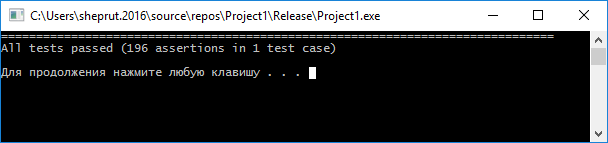
\includegraphics[scale=0.7]{unit_test.png}
\end{center}

\section{Исследования}

\subsection{Матрица с диагональным преобладанием}
$$ A=\left(\quad\begin{matrix}
\cellcolor{green!30}2 & \cellcolor{green!30}0 & 0 & 0 & \cellcolor{green!30}0 & 0 & \cellcolor{green!30}-1 & 0 & 0 & 0 \\
\cellcolor{green!30}-3 & \cellcolor{green!30}13 & \cellcolor{green!30}-4 & 0 & 0 & \cellcolor{green!30}-4 & 0 & \cellcolor{green!30}-2 & 0 & 0 \\
0 & \cellcolor{green!30}0 & \cellcolor{green!30}7 & \cellcolor{green!30}-3 & 0 & 0 & \cellcolor{green!30}-2 & 0 & \cellcolor{green!30}-2 & 0 \\
0 & 0 & \cellcolor{green!30}-3 & \cellcolor{green!30}8 & \cellcolor{green!30}-2 & 0 & 0 & \cellcolor{green!30}0 & 0 & \cellcolor{green!30}-3 \\
\cellcolor{green!30}-2 & 0 & 0 & \cellcolor{green!30}-2 & \cellcolor{green!30}5 & \cellcolor{green!30}-1 & 0 & 0 & \cellcolor{green!30}0 & 0 \\
0 & \cellcolor{green!30}-1 & 0 & 0 & \cellcolor{green!30}-1 & \cellcolor{green!30}2 & \cellcolor{green!30}0 & 0 & 0 & \cellcolor{green!30}0 \\
\cellcolor{green!30}-2 & 0 & \cellcolor{green!30}-4 & 0 & 0 & \cellcolor{green!30}0 & \cellcolor{green!30}6 & \cellcolor{green!30}0 & 0 & 0 \\
0 & \cellcolor{green!30}0 & 0 & \cellcolor{green!30}-3 & 0 & 0 & \cellcolor{green!30}-3 & \cellcolor{green!30}7 & \cellcolor{green!30}-1 & 0 \\
0 & 0 & \cellcolor{green!30}-2 & 0 & \cellcolor{green!30}-4 & 0 & 0 & \cellcolor{green!30}-3 & \cellcolor{green!30}9 & \cellcolor{green!30}0 \\
0 & 0 & 0 & \cellcolor{green!30}-1 & 0 & \cellcolor{green!30}-4 & 0 & 0 & \cellcolor{green!30}-4 & \cellcolor{green!30}9 
\end{matrix}\quad\right), X=\begin{pmatrix}1 \\
2 \\
3 \\
4 \\
5 \\
6 \\
7 \\
8 \\
9 \\
10 
\end{pmatrix}, F=\begin{pmatrix}-5 \\
-29 \\
-23 \\
-17 \\
9 \\
5 \\
28 \\
14 \\
31 \\
26 
\end{pmatrix} $$

$$ \varepsilon = 10^{-14}, \quad iterations_{max} = 100000, \quad start = \begin{pmatrix} 0 & 0 & 0 & 0 & 0 & 0 & 0 & 0 & 0 & 0 \end{pmatrix}^T $$

\setlength{\tabcolsep}{2pt}
\tabulinesep=0.3mm
\noindent{\scriptsize\texttt{\begin{longtabu}{
|X[-1,c]||X[-1,c]|X[-1,c]|X[-1,c]|X[-1,c]|X[-1,c]|
p{0.05cm}
|X[-1,c]||X[-1,c]|X[-1,c]|X[-1,c]|X[-1,c]|X[-1,c]|}
\cline{1-6}\cline{8-13}
\multicolumn{6}{|c|}{Метод Якоби} && \multicolumn{6}{c|}{Метод Зейделя} \\
\hhline{*{6}{-}~*{6}{-}}
$w$ & $x$ & $x-x^*$ & \tcell{\tiny Относительная\\\tiny невязка} & {\tiny $\mathop{cond}(A) >$} & {\tiny Итераций} && $w$ & $x$ & $x-x^*$ & \tcell{\tiny Относительная\\\tiny невязка} & {\tiny $\mathop{cond}(A) >$} & {\tiny Итераций} \\
\hhline{*{6}{-}~*{6}{-}}
0.10 & \tiny{\tcell{0.9999999999997312 \\ 1.9999999999994800 \\ 2.9999999999994125 \\ 3.9999999999994142 \\ 4.9999999999995302 \\ 5.9999999999994751 \\ 6.9999999999994902 \\ 7.9999999999994200 \\ 8.9999999999994404 \\ 9.9999999999994262}} & \tiny{\tcell{2.7e-13 \\ 5.2e-13 \\ 5.9e-13 \\ 5.9e-13 \\ 4.7e-13 \\ 5.2e-13 \\ 5.1e-13 \\ 5.8e-13 \\ 5.6e-13 \\ 5.7e-13}} & 9.9e-15 & 8.54 & 5678 &  & 0.10 & \tiny{\tcell{0.9999999999997365 \\ 1.9999999999994895 \\ 2.9999999999994222 \\ 3.9999999999994245 \\ 4.9999999999995381 \\ 5.9999999999994866 \\ 6.9999999999995008 \\ 7.9999999999994333 \\ 8.9999999999994529 \\ 9.9999999999994351}} & \tiny{\tcell{2.6e-13 \\ 5.1e-13 \\ 5.8e-13 \\ 5.8e-13 \\ 4.6e-13 \\ 5.1e-13 \\ 5.0e-13 \\ 5.7e-13 \\ 5.5e-13 \\ 5.6e-13}} & 9.9e-15 & 8.36 & 5381 \\
\hhline{*{6}{-}~*{6}{-}}
0.20 & \tiny{\tcell{0.9999999999997413 \\ 1.9999999999994982 \\ 2.9999999999994329 \\ 3.9999999999994347 \\ 4.9999999999995453 \\ 5.9999999999994946 \\ 6.9999999999995097 \\ 7.9999999999994413 \\ 8.9999999999994564 \\ 9.9999999999994404}} & \tiny{\tcell{2.6e-13 \\ 5.0e-13 \\ 5.7e-13 \\ 5.7e-13 \\ 4.5e-13 \\ 5.1e-13 \\ 4.9e-13 \\ 5.6e-13 \\ 5.4e-13 \\ 5.6e-13}} & 1.0e-14 & 8.22 & 2833 &  & 0.20 & \tiny{\tcell{0.9999999999997410 \\ 1.9999999999994977 \\ 2.9999999999994329 \\ 3.9999999999994373 \\ 4.9999999999995479 \\ 5.9999999999994991 \\ 6.9999999999995124 \\ 7.9999999999994458 \\ 8.9999999999994635 \\ 9.9999999999994511}} & \tiny{\tcell{2.6e-13 \\ 5.0e-13 \\ 5.7e-13 \\ 5.6e-13 \\ 4.5e-13 \\ 5.0e-13 \\ 4.9e-13 \\ 5.5e-13 \\ 5.4e-13 \\ 5.5e-13}} & 9.9e-15 & 8.19 & 2532 \\
\hhline{*{6}{-}~*{6}{-}}
0.30 & \tiny{\tcell{0.9999999999997444 \\ 1.9999999999995042 \\ 2.9999999999994396 \\ 3.9999999999994413 \\ 4.9999999999995506 \\ 5.9999999999995008 \\ 6.9999999999995159 \\ 7.9999999999994476 \\ 8.9999999999994635 \\ 9.9999999999994476}} & \tiny{\tcell{2.6e-13 \\ 5.0e-13 \\ 5.6e-13 \\ 5.6e-13 \\ 4.5e-13 \\ 5.0e-13 \\ 4.8e-13 \\ 5.5e-13 \\ 5.4e-13 \\ 5.5e-13}} & 9.9e-15 & 8.21 & 1884 &  & 0.30 & \tiny{\tcell{0.9999999999997394 \\ 1.9999999999994948 \\ 2.9999999999994307 \\ 3.9999999999994369 \\ 4.9999999999995488 \\ 5.9999999999994991 \\ 6.9999999999995115 \\ 7.9999999999994467 \\ 8.9999999999994653 \\ 9.9999999999994529}} & \tiny{\tcell{2.6e-13 \\ 5.1e-13 \\ 5.7e-13 \\ 5.6e-13 \\ 4.5e-13 \\ 5.0e-13 \\ 4.9e-13 \\ 5.5e-13 \\ 5.3e-13 \\ 5.5e-13}} & 1.0e-14 & 8.14 & 1582 \\
\hhline{*{6}{-}~*{6}{-}}
0.40 & \tiny{\tcell{0.9999999999997434 \\ 1.9999999999995017 \\ 2.9999999999994365 \\ 3.9999999999994382 \\ 4.9999999999995488 \\ 5.9999999999994991 \\ 6.9999999999995133 \\ 7.9999999999994449 \\ 8.9999999999994618 \\ 9.9999999999994458}} & \tiny{\tcell{2.6e-13 \\ 5.0e-13 \\ 5.6e-13 \\ 5.6e-13 \\ 4.5e-13 \\ 5.0e-13 \\ 4.9e-13 \\ 5.6e-13 \\ 5.4e-13 \\ 5.5e-13}} & 9.9e-15 & 8.21 & 1409 &  & 0.40 & \tiny{\tcell{0.9999999999997397 \\ 1.9999999999994955 \\ 2.9999999999994316 \\ 3.9999999999994396 \\ 4.9999999999995506 \\ 5.9999999999995026 \\ 6.9999999999995142 \\ 7.9999999999994511 \\ 8.9999999999994689 \\ 9.9999999999994582}} & \tiny{\tcell{2.6e-13 \\ 5.0e-13 \\ 5.7e-13 \\ 5.6e-13 \\ 4.5e-13 \\ 5.0e-13 \\ 4.9e-13 \\ 5.5e-13 \\ 5.3e-13 \\ 5.4e-13}} & 1.0e-14 & 8.10 & 1107 \\
\hhline{*{6}{-}~*{6}{-}}
0.50 & \tiny{\tcell{0.9999999999997422 \\ 1.9999999999994995 \\ 2.9999999999994347 \\ 3.9999999999994369 \\ 4.9999999999995470 \\ 5.9999999999994973 \\ 6.9999999999995115 \\ 7.9999999999994422 \\ 8.9999999999994582 \\ 9.9999999999994440}} & \tiny{\tcell{2.6e-13 \\ 5.0e-13 \\ 5.7e-13 \\ 5.6e-13 \\ 4.5e-13 \\ 5.0e-13 \\ 4.9e-13 \\ 5.6e-13 \\ 5.4e-13 \\ 5.6e-13}} & 9.9e-15 & 8.21 & 1124 &  & 0.50 & \tiny{\tcell{0.9999999999997498 \\ 1.9999999999995155 \\ 2.9999999999994547 \\ 3.9999999999994644 \\ 4.9999999999995710 \\ 5.9999999999995257 \\ 6.9999999999995355 \\ 7.9999999999994778 \\ 8.9999999999994955 \\ 9.9999999999994866}} & \tiny{\tcell{2.5e-13 \\ 4.8e-13 \\ 5.5e-13 \\ 5.4e-13 \\ 4.3e-13 \\ 4.7e-13 \\ 4.6e-13 \\ 5.2e-13 \\ 5.0e-13 \\ 5.1e-13}} & 9.8e-15 & 7.92 & 823 \\
\hhline{*{6}{-}~*{6}{-}}
0.60 & \tiny{\tcell{0.9999999999997411 \\ 1.9999999999994975 \\ 2.9999999999994320 \\ 3.9999999999994347 \\ 4.9999999999995453 \\ 5.9999999999994946 \\ 6.9999999999995097 \\ 7.9999999999994404 \\ 8.9999999999994564 \\ 9.9999999999994422}} & \tiny{\tcell{2.6e-13 \\ 5.0e-13 \\ 5.7e-13 \\ 5.7e-13 \\ 4.5e-13 \\ 5.1e-13 \\ 4.9e-13 \\ 5.6e-13 \\ 5.4e-13 \\ 5.6e-13}} & 9.9e-15 & 8.29 & 934 &  & 0.60 & \tiny{\tcell{0.9999999999997568 \\ 1.9999999999995293 \\ 2.9999999999994706 \\ 3.9999999999994831 \\ 4.9999999999995870 \\ 5.9999999999995435 \\ 6.9999999999995524 \\ 7.9999999999994973 \\ 8.9999999999995168 \\ 9.9999999999995097}} & \tiny{\tcell{2.4e-13 \\ 4.7e-13 \\ 5.3e-13 \\ 5.2e-13 \\ 4.1e-13 \\ 4.6e-13 \\ 4.5e-13 \\ 5.0e-13 \\ 4.8e-13 \\ 4.9e-13}} & 9.7e-15 & 7.69 & 633 \\
\hhline{*{6}{-}~*{6}{-}}
0.70 & \tiny{\tcell{0.9999999999997469 \\ 1.9999999999995088 \\ 2.9999999999994449 \\ 3.9999999999994476 \\ 4.9999999999995559 \\ 5.9999999999995062 \\ 6.9999999999995204 \\ 7.9999999999994520 \\ 8.9999999999994689 \\ 9.9999999999994547}} & \tiny{\tcell{2.5e-13 \\ 4.9e-13 \\ 5.6e-13 \\ 5.5e-13 \\ 4.4e-13 \\ 4.9e-13 \\ 4.8e-13 \\ 5.5e-13 \\ 5.3e-13 \\ 5.5e-13}} & 9.6e-15 & 8.31 & 799 &  & 0.70 & \tiny{\tcell{0.9999999999997663 \\ 1.9999999999995477 \\ 2.9999999999994920 \\ 3.9999999999995066 \\ 4.9999999999996056 \\ 5.9999999999995648 \\ 6.9999999999995719 \\ 7.9999999999995230 \\ 8.9999999999995399 \\ 9.9999999999995346}} & \tiny{\tcell{2.3e-13 \\ 4.5e-13 \\ 5.1e-13 \\ 4.9e-13 \\ 3.9e-13 \\ 4.4e-13 \\ 4.3e-13 \\ 4.8e-13 \\ 4.6e-13 \\ 4.7e-13}} & 9.5e-15 & 7.46 & 497 \\
\hhline{*{6}{-}~*{6}{-}}
0.80 & \tiny{\tcell{0.9999999999997445 \\ 1.9999999999995040 \\ 2.9999999999994396 \\ 3.9999999999994413 \\ 4.9999999999995515 \\ 5.9999999999995008 \\ 6.9999999999995159 \\ 7.9999999999994476 \\ 8.9999999999994618 \\ 9.9999999999994493}} & \tiny{\tcell{2.6e-13 \\ 5.0e-13 \\ 5.6e-13 \\ 5.6e-13 \\ 4.5e-13 \\ 5.0e-13 \\ 4.8e-13 \\ 5.5e-13 \\ 5.4e-13 \\ 5.5e-13}} & 9.8e-15 & 8.23 & 697 &  & 0.80 & \tiny{\tcell{0.9999999999997817 \\ 1.9999999999995768 \\ 2.9999999999995257 \\ 3.9999999999995417 \\ 4.9999999999996350 \\ 5.9999999999995977 \\ 6.9999999999996039 \\ 7.9999999999995604 \\ 8.9999999999995772 \\ 9.9999999999995737}} & \tiny{\tcell{2.2e-13 \\ 4.2e-13 \\ 4.7e-13 \\ 4.6e-13 \\ 3.7e-13 \\ 4.0e-13 \\ 4.0e-13 \\ 4.4e-13 \\ 4.2e-13 \\ 4.3e-13}} & 9.4e-15 & 6.99 & 395 \\
\hhline{*{6}{-}~*{6}{-}}
0.90 & \tiny{\tcell{0.9999999999997456 \\ 1.9999999999995062 \\ 2.9999999999994418 \\ 3.9999999999994440 \\ 4.9999999999995532 \\ 5.9999999999995035 \\ 6.9999999999995186 \\ 7.9999999999994502 \\ 8.9999999999994671 \\ 9.9999999999994511}} & \tiny{\tcell{2.5e-13 \\ 4.9e-13 \\ 5.6e-13 \\ 5.6e-13 \\ 4.5e-13 \\ 5.0e-13 \\ 4.8e-13 \\ 5.5e-13 \\ 5.3e-13 \\ 5.5e-13}} & 9.8e-15 & 8.17 & 618 &  & 0.90 & \tiny{\tcell{0.9999999999997934 \\ 1.9999999999996005 \\ 2.9999999999995537 \\ 3.9999999999995723 \\ 4.9999999999996607 \\ 5.9999999999996261 \\ 6.9999999999996296 \\ 7.9999999999995932 \\ 8.9999999999996092 \\ 9.9999999999996074}} & \tiny{\tcell{2.1e-13 \\ 4.0e-13 \\ 4.5e-13 \\ 4.3e-13 \\ 3.4e-13 \\ 3.7e-13 \\ 3.7e-13 \\ 4.1e-13 \\ 3.9e-13 \\ 3.9e-13}} & 9.5e-15 & 6.43 & 315 \\
\hhline{*{6}{-}~*{6}{-}}
1.00 & \tiny{\tcell{0.9999999999997509 \\ 1.9999999999995151 \\ 2.9999999999994529 \\ 3.9999999999994547 \\ 4.9999999999995612 \\ 5.9999999999995133 \\ 6.9999999999995266 \\ 7.9999999999994609 \\ 8.9999999999994760 \\ 9.9999999999994618}} & \tiny{\tcell{2.5e-13 \\ 4.8e-13 \\ 5.5e-13 \\ 5.5e-13 \\ 4.4e-13 \\ 4.9e-13 \\ 4.7e-13 \\ 5.4e-13 \\ 5.2e-13 \\ 5.4e-13}} & 9.7e-15 & 8.14 & 555 &  & 1.00 & \tiny{\tcell{0.9999999999998201 \\ 1.9999999999996521 \\ 2.9999999999996123 \\ 3.9999999999996323 \\ 4.9999999999997087 \\ 5.9999999999996803 \\ 6.9999999999996820 \\ 7.9999999999996536 \\ 8.9999999999996678 \\ 9.9999999999996696}} & \tiny{\tcell{1.8e-13 \\ 3.5e-13 \\ 3.9e-13 \\ 3.7e-13 \\ 2.9e-13 \\ 3.2e-13 \\ 3.2e-13 \\ 3.5e-13 \\ 3.3e-13 \\ 3.3e-13}} & 9.0e-15 & 5.84 & 251 \\
\hhline{*{6}{-}~*{6}{-}}
\cellcolor{orange!30}{1.07} & \tiny{\cellcolor{orange!30}{\tcell{0.9999999999997543 \\ 1.9999999999995248 \\ 2.9999999999994631 \\ 3.9999999999994653 \\ 4.9999999999995692 \\ 5.9999999999995222 \\ 6.9999999999995355 \\ 7.9999999999994698 \\ 8.9999999999994849 \\ 9.9999999999994724}}} & \tiny{\cellcolor{orange!30}{\tcell{2.5e-13 \\ 4.8e-13 \\ 5.4e-13 \\ 5.3e-13 \\ 4.3e-13 \\ 4.8e-13 \\ 4.6e-13 \\ 5.3e-13 \\ 5.2e-13 \\ 5.3e-13}}} & \cellcolor{orange!30}{9.4e-15} & \cellcolor{orange!30}{8.26} & \cellcolor{orange!30}{518} &  & 1.07 & \tiny{\tcell{0.9999999999998176 \\ 1.9999999999996478 \\ 2.9999999999996079 \\ 3.9999999999996327 \\ 4.9999999999997087 \\ 5.9999999999996820 \\ 6.9999999999996811 \\ 7.9999999999996554 \\ 8.9999999999996732 \\ 9.9999999999996749}} & \tiny{\tcell{1.8e-13 \\ 3.5e-13 \\ 3.9e-13 \\ 3.7e-13 \\ 2.9e-13 \\ 3.2e-13 \\ 3.2e-13 \\ 3.4e-13 \\ 3.3e-13 \\ 3.3e-13}} & 9.9e-15 & 5.32 & 212 \\
\hhline{*{6}{-}~*{6}{-}}
\cellcolor{green!30}{1.08} & \tiny{\cellcolor{green!30}{\tcell{0.9999999999997538 \\ 1.9999999999995233 \\ 2.9999999999994595 \\ 3.9999999999994640 \\ 4.9999999999995683 \\ 5.9999999999995204 \\ 6.9999999999995355 \\ 7.9999999999994680 \\ 8.9999999999994831 \\ 9.9999999999994706}}} & \tiny{\cellcolor{green!30}{\tcell{2.5e-13 \\ 4.8e-13 \\ 5.4e-13 \\ 5.4e-13 \\ 4.3e-13 \\ 4.8e-13 \\ 4.6e-13 \\ 5.3e-13 \\ 5.2e-13 \\ 5.3e-13}}} & \cellcolor{green!30}{9.3e-15} & \cellcolor{green!30}{8.35} & \cellcolor{green!30}{513} &  & 1.08 & \tiny{\tcell{0.9999999999998229 \\ 1.9999999999996569 \\ 2.9999999999996190 \\ 3.9999999999996430 \\ 4.9999999999997176 \\ 5.9999999999996909 \\ 6.9999999999996900 \\ 7.9999999999996643 \\ 8.9999999999996803 \\ 9.9999999999996856}} & \tiny{\tcell{1.8e-13 \\ 3.4e-13 \\ 3.8e-13 \\ 3.6e-13 \\ 2.8e-13 \\ 3.1e-13 \\ 3.1e-13 \\ 3.4e-13 \\ 3.2e-13 \\ 3.1e-13}} & 9.6e-15 & 5.30 & 207 \\
\hhline{*{6}{-}~*{6}{-}}
\cellcolor{orange!30}{1.09} & \tiny{\cellcolor{orange!30}{\tcell{1.0000000000000042 \\ 1.9999999999999687 \\ 2.9999999999999876 \\ 4.0000000000000027 \\ 4.9999999999999689 \\ 6.0000000000000195 \\ 6.9999999999999796 \\ 7.9999999999999911 \\ 8.9999999999999947 \\ 9.9999999999999662}}} & \tiny{\cellcolor{orange!30}{\tcell{-4.2e-15 \\ 3.1e-14 \\ 1.2e-14 \\ -2.7e-15 \\ 3.1e-14 \\ -2.0e-14 \\ 2.0e-14 \\ 8.9e-15 \\ 5.3e-15 \\ 3.4e-14}}} & \cellcolor{orange!30}{1.0e-14} & \cellcolor{orange!30}{0.33} & \cellcolor{orange!30}{573} &  & 1.09 & \tiny{\tcell{0.9999999999998253 \\ 1.9999999999996623 \\ 2.9999999999996239 \\ 3.9999999999996474 \\ 4.9999999999997220 \\ 5.9999999999996962 \\ 6.9999999999996945 \\ 7.9999999999996705 \\ 8.9999999999996891 \\ 9.9999999999996909}} & \tiny{\tcell{1.7e-13 \\ 3.4e-13 \\ 3.8e-13 \\ 3.5e-13 \\ 2.8e-13 \\ 3.0e-13 \\ 3.1e-13 \\ 3.3e-13 \\ 3.1e-13 \\ 3.1e-13}} & 9.6e-15 & 5.22 & 202 \\
\hhline{*{6}{-}~*{6}{-}}
1.10 & \tiny{\tcell{1.0000000000000113 \\ 1.9999999999999800 \\ 3.0000000000000013 \\ 4.0000000000000124 \\ 4.9999999999999813 \\ 6.0000000000000284 \\ 6.9999999999999893 \\ 8.0000000000000053 \\ 9.0000000000000053 \\ 9.9999999999999822}} & \tiny{\tcell{-1.1e-14 \\ 2.0e-14 \\ -1.3e-15 \\ -1.2e-14 \\ 1.9e-14 \\ -2.8e-14 \\ 1.1e-14 \\ -5.3e-15 \\ -5.3e-15 \\ 1.8e-14}} & 9.1e-15 & 0.27 & 875 &  & 1.10 & \tiny{\tcell{0.9999999999998258 \\ 1.9999999999996636 \\ 2.9999999999996265 \\ 3.9999999999996509 \\ 4.9999999999997247 \\ 5.9999999999996989 \\ 6.9999999999996971 \\ 7.9999999999996723 \\ 8.9999999999996891 \\ 9.9999999999996927}} & \tiny{\tcell{1.7e-13 \\ 3.4e-13 \\ 3.7e-13 \\ 3.5e-13 \\ 2.8e-13 \\ 3.0e-13 \\ 3.0e-13 \\ 3.3e-13 \\ 3.1e-13 \\ 3.1e-13}} & 9.6e-15 & 5.19 & 197 \\
\hhline{*{6}{-}~*{6}{-}}
& & & & & & & 1.20 & \tiny{\tcell{0.9999999999998664 \\ 1.9999999999997420 \\ 2.9999999999997149 \\ 3.9999999999997380 \\ 4.9999999999997948 \\ 5.9999999999997771 \\ 6.9999999999997735 \\ 7.9999999999997611 \\ 8.9999999999997744 \\ 9.9999999999997797}} & \tiny{\tcell{1.3e-13 \\ 2.6e-13 \\ 2.9e-13 \\ 2.6e-13 \\ 2.1e-13 \\ 2.2e-13 \\ 2.3e-13 \\ 2.4e-13 \\ 2.3e-13 \\ 2.2e-13}} & 8.7e-15 & 4.28 & 152 \\
\hhline{*{6}{-}~*{6}{-}}
& & & & & & & 1.30 & \tiny{\tcell{0.9999999999998852 \\ 1.9999999999997773 \\ 2.9999999999997558 \\ 3.9999999999997824 \\ 4.9999999999998312 \\ 5.9999999999998179 \\ 6.9999999999998126 \\ 7.9999999999998055 \\ 8.9999999999998206 \\ 9.9999999999998295}} & \tiny{\tcell{1.1e-13 \\ 2.2e-13 \\ 2.4e-13 \\ 2.2e-13 \\ 1.7e-13 \\ 1.8e-13 \\ 1.9e-13 \\ 1.9e-13 \\ 1.8e-13 \\ 1.7e-13}} & 9.3e-15 & 3.31 & 111 \\
\hhline{*{6}{-}~*{6}{-}}
& & & & & & & \cellcolor{orange!30}{1.36} & \tiny{\cellcolor{orange!30}{\tcell{0.9999999999999248 \\ 1.9999999999998550 \\ 2.9999999999998419 \\ 3.9999999999998672 \\ 4.9999999999998979 \\ 5.9999999999998881 \\ 6.9999999999998828 \\ 7.9999999999998854 \\ 8.9999999999998952 \\ 9.9999999999999005}}} & \tiny{\cellcolor{orange!30}{\tcell{7.5e-14 \\ 1.4e-13 \\ 1.6e-13 \\ 1.3e-13 \\ 1.0e-13 \\ 1.1e-13 \\ 1.2e-13 \\ 1.1e-13 \\ 1.0e-13 \\ 9.9e-14}}} & \cellcolor{orange!30}{7.4e-15} & \cellcolor{orange!30}{2.59} & \cellcolor{orange!30}{88} \\
\hhline{*{6}{-}~*{6}{-}}
& & & & & & & \cellcolor{green!30}{1.37} & \tiny{\cellcolor{green!30}{\tcell{0.9999999999999157 \\ 1.9999999999998914 \\ 2.9999999999998836 \\ 3.9999999999999565 \\ 4.9999999999999458 \\ 5.9999999999998996 \\ 6.9999999999998996 \\ 7.9999999999999503 \\ 8.9999999999999432 \\ 9.9999999999999130}}} & \tiny{\cellcolor{green!30}{\tcell{8.4e-14 \\ 1.1e-13 \\ 1.2e-13 \\ 4.4e-14 \\ 5.4e-14 \\ 1.0e-13 \\ 1.0e-13 \\ 5.0e-14 \\ 5.7e-14 \\ 8.7e-14}}} & \cellcolor{green!30}{9.1e-15} & \cellcolor{green!30}{1.49} & \cellcolor{green!30}{85} \\
\hhline{*{6}{-}~*{6}{-}}
& & & & & & & \cellcolor{orange!30}{1.38} & \tiny{\cellcolor{orange!30}{\tcell{1.0000000000000264 \\ 2.0000000000000280 \\ 2.9999999999999640 \\ 4.0000000000000036 \\ 5.0000000000000364 \\ 6.0000000000000373 \\ 6.9999999999999574 \\ 7.9999999999999813 \\ 9.0000000000000107 \\ 10.0000000000000195}}} & \tiny{\cellcolor{orange!30}{\tcell{-2.6e-14 \\ -2.8e-14 \\ 3.6e-14 \\ -3.6e-15 \\ -3.6e-14 \\ -3.7e-14 \\ 4.3e-14 \\ 1.9e-14 \\ -1.1e-14 \\ -2.0e-14}}} & \cellcolor{orange!30}{6.6e-15} & \cellcolor{orange!30}{0.70} & \cellcolor{orange!30}{90} \\
\hhline{*{6}{-}~*{6}{-}}
& & & & & & & 1.40 & \tiny{\tcell{1.0000000000000024 \\ 1.9999999999999885 \\ 3.0000000000000351 \\ 3.9999999999999760 \\ 4.9999999999999698 \\ 5.9999999999999920 \\ 7.0000000000000480 \\ 8.0000000000000018 \\ 8.9999999999999876 \\ 10.0000000000000000}} & \tiny{\tcell{-2.4e-15 \\ 1.2e-14 \\ -3.5e-14 \\ 2.4e-14 \\ 3.0e-14 \\ 8.0e-15 \\ -4.8e-14 \\ -1.8e-15 \\ 1.2e-14 \\ 0.0e+00}} & 7.3e-15 & 0.51 & 103 \\
\hhline{*{6}{-}~*{6}{-}}
& & & & & & & 1.50 & \tiny{\tcell{0.9999999999999558 \\ 1.9999999999999600 \\ 3.0000000000000373 \\ 4.0000000000000036 \\ 4.9999999999999520 \\ 5.9999999999999396 \\ 7.0000000000000524 \\ 8.0000000000000355 \\ 8.9999999999999840 \\ 9.9999999999999556}} & \tiny{\tcell{4.4e-14 \\ 4.0e-14 \\ -3.7e-14 \\ -3.6e-15 \\ 4.8e-14 \\ 6.0e-14 \\ -5.2e-14 \\ -3.6e-14 \\ 1.6e-14 \\ 4.4e-14}} & 8.5e-15 & 0.79 & 285 \\
\hhline{*{6}{-}~*{6}{-}}
\end{longtabu}}}

\subsubsection{График зависимости числа итераций от параметра релаксации}

\noindent\begin{tikzpicture}
\begin{semilogyaxis}[xlabel=w,ylabel=Итераций,width=\textwidth, height=6cm]
\addplot[red, no markers] table [y=it1, x=w1]{A.dat};
\addplot[blue, no markers] table [y=it2, x=w2]{A.dat};
\legend{Метод Якоби,Метод Зейделя}
\end{semilogyaxis}
\end{tikzpicture}

\subsubsection{Расчет числа обусловленности через MathCad}
$\displaystyle
	\begin{aligned}
		&\mathop{conde}(A) = 133.86 \\
		&\mathop{condi}(A) = 111.728 \\
		&\mathop{conde}(A) = 200  \\
		&\mathop{conde}(A) = 74.622  \\
		&\frac{\lambda^A_{max}}{\lambda^A_{min}} = \frac{13.709}{0.278} = 49.313  \\
	\end{aligned}
$

\subsection{Матрица с обратным знаком внедиагональных элементов}
$$ B=\left(\quad\begin{matrix}
\cellcolor{green!30}9 & \cellcolor{green!30}4 & 0 & \cellcolor{green!30}1 & 0 & 0 & 0 & \cellcolor{green!30}3 & 0 & 0 \\
\cellcolor{green!30}4 & \cellcolor{green!30}8 & \cellcolor{green!30}0 & 0 & \cellcolor{green!30}2 & 0 & 0 & 0 & \cellcolor{green!30}2 & 0 \\
0 & \cellcolor{green!30}3 & \cellcolor{green!30}9 & \cellcolor{green!30}1 & 0 & \cellcolor{green!30}3 & 0 & 0 & 0 & \cellcolor{green!30}2 \\
\cellcolor{green!30}0 & 0 & \cellcolor{green!30}0 & \cellcolor{green!30}4 & \cellcolor{green!30}0 & 0 & \cellcolor{green!30}4 & 0 & 0 & 0 \\
0 & \cellcolor{green!30}1 & 0 & \cellcolor{green!30}2 & \cellcolor{green!30}9 & \cellcolor{green!30}3 & 0 & \cellcolor{green!30}3 & 0 & 0 \\
0 & 0 & \cellcolor{green!30}2 & 0 & \cellcolor{green!30}1 & \cellcolor{green!30}5 & \cellcolor{green!30}0 & 0 & \cellcolor{green!30}2 & 0 \\
0 & 0 & 0 & \cellcolor{green!30}4 & 0 & \cellcolor{green!30}3 & \cellcolor{green!30}8 & \cellcolor{green!30}0 & 0 & \cellcolor{green!30}1 \\
\cellcolor{green!30}1 & 0 & 0 & 0 & \cellcolor{green!30}2 & 0 & \cellcolor{green!30}3 & \cellcolor{green!30}10 & \cellcolor{green!30}4 & 0 \\
0 & \cellcolor{green!30}0 & 0 & 0 & 0 & \cellcolor{green!30}4 & 0 & \cellcolor{green!30}2 & \cellcolor{green!30}7 & \cellcolor{green!30}1 \\
0 & 0 & \cellcolor{green!30}3 & 0 & 0 & 0 & \cellcolor{green!30}3 & 0 & \cellcolor{green!30}1 & \cellcolor{green!30}7 
\end{matrix}\quad\right), X=\begin{pmatrix}1 \\
2 \\
3 \\
4 \\
5 \\
6 \\
7 \\
8 \\
9 \\
10 
\end{pmatrix}, F=\begin{pmatrix}45 \\
48 \\
75 \\
44 \\
97 \\
59 \\
100 \\
148 \\
113 \\
109 
\end{pmatrix} $$

$$ \varepsilon = 10^{-14}, \quad iterations_{max} = 100000, \quad start = \begin{pmatrix} 0 & 0 & 0 & 0 & 0 & 0 & 0 & 0 & 0 & 0 \end{pmatrix}^T $$

\setlength{\tabcolsep}{2pt}
\tabulinesep=0.3mm
\noindent{\scriptsize\texttt{\begin{longtabu}{
|X[-1,c]||X[-1,c]|X[-1,c]|X[-1,c]|X[-1,c]|X[-1,c]|
p{0.05cm}
|X[-1,c]||X[-1,c]|X[-1,c]|X[-1,c]|X[-1,c]|X[-1,c]|}
\cline{1-6}\cline{8-13}
\multicolumn{6}{|c|}{Метод Якоби} && \multicolumn{6}{c|}{Метод Зейделя} \\
\cline{1-6}\cline{8-13}
0.00 & \tiny{\tcell{0.0000000000000000 \\ 0.0000000000000000 \\ 0.0000000000000000 \\ 0.0000000000000000 \\ 0.0000000000000000 \\ 0.0000000000000000 \\ 0.0000000000000000 \\ 0.0000000000000000 \\ 0.0000000000000000 \\ 0.0000000000000000}} & \tiny{\tcell{1.00e+00 \\ 2.00e+00 \\ 3.00e+00 \\ 4.00e+00 \\ 5.00e+00 \\ 6.00e+00 \\ 7.00e+00 \\ 8.00e+00 \\ 9.00e+00 \\ 1.00e+01}} & 1.00e+00 & 1.00 & 100000 &  & 0.00 & \tiny{\tcell{0.0000000000000000 \\ 0.0000000000000000 \\ 0.0000000000000000 \\ 0.0000000000000000 \\ 0.0000000000000000 \\ 0.0000000000000000 \\ 0.0000000000000000 \\ 0.0000000000000000 \\ 0.0000000000000000 \\ 0.0000000000000000}} & \tiny{\tcell{1.0e+00 \\ 2.0e+00 \\ 3.0e+00 \\ 4.0e+00 \\ 5.0e+00 \\ 6.0e+00 \\ 7.0e+00 \\ 8.0e+00 \\ 9.0e+00 \\ 1.0e+01}} & 1.00e+00 & 1.00 & 100000 \\
\cline{1-6}\cline{8-13}
0.10 & \tiny{\tcell{0.9999999999748445 \\ 2.0000000000272502 \\ 2.9999999999713296 \\ 4.0000000000295977 \\ 4.9999999999709344 \\ 6.0000000000290692 \\ 6.9999999999705302 \\ 8.0000000000289546 \\ 8.9999999999708287 \\ 10.0000000000291998}} & \tiny{\tcell{2.52e-11 \\ -2.73e-11 \\ 2.87e-11 \\ -2.96e-11 \\ 2.91e-11 \\ -2.91e-11 \\ 2.95e-11 \\ -2.90e-11 \\ 2.92e-11 \\ -2.92e-11}} & 9.99e-15 & 461.37 & 52448 &  & 0.10 & \tiny{\tcell{0.9999999999750441 \\ 2.0000000000270322 \\ 2.9999999999715627 \\ 4.0000000000293552 \\ 4.9999999999711697 \\ 6.0000000000288320 \\ 6.9999999999707736 \\ 8.0000000000287201 \\ 8.9999999999710614 \\ 10.0000000000289617}} & \tiny{\tcell{2.5e-11 \\ -2.7e-11 \\ 2.8e-11 \\ -2.9e-11 \\ 2.9e-11 \\ -2.9e-11 \\ 2.9e-11 \\ -2.9e-11 \\ 2.9e-11 \\ -2.9e-11}} & 9.99e-15 & 457.30 & 51082 \\
\cline{1-6}\cline{8-13}
0.20 & \tiny{\tcell{0.9999999999751141 \\ 2.0000000000269584 \\ 2.9999999999716391 \\ 4.0000000000292735 \\ 4.9999999999712452 \\ 6.0000000000287601 \\ 6.9999999999708482 \\ 8.0000000000286509 \\ 8.9999999999711324 \\ 10.0000000000288924}} & \tiny{\tcell{2.49e-11 \\ -2.70e-11 \\ 2.84e-11 \\ -2.93e-11 \\ 2.88e-11 \\ -2.88e-11 \\ 2.92e-11 \\ -2.87e-11 \\ 2.89e-11 \\ -2.89e-11}} & 9.98e-15 & 456.98 & 26225 &  & 0.20 & \tiny{\tcell{0.9999999999751906 \\ 2.0000000000268678 \\ 2.9999999999717359 \\ 4.0000000000291758 \\ 4.9999999999713474 \\ 6.0000000000286517 \\ 6.9999999999709601 \\ 8.0000000000285354 \\ 8.9999999999712532 \\ 10.0000000000287717}} & \tiny{\tcell{2.5e-11 \\ -2.7e-11 \\ 2.8e-11 \\ -2.9e-11 \\ 2.9e-11 \\ -2.9e-11 \\ 2.9e-11 \\ -2.9e-11 \\ 2.9e-11 \\ -2.9e-11}} & 1.00e-14 & 454.29 & 24500 \\
\cline{1-6}\cline{8-13}
0.30 & \tiny{\tcell{0.9999999999749128 \\ 2.0000000000271765 \\ 2.9999999999714091 \\ 4.0000000000295106 \\ 4.9999999999710134 \\ 6.0000000000289937 \\ 6.9999999999706111 \\ 8.0000000000288818 \\ 8.9999999999708997 \\ 10.0000000000291251}} & \tiny{\tcell{2.51e-11 \\ -2.72e-11 \\ 2.86e-11 \\ -2.95e-11 \\ 2.90e-11 \\ -2.90e-11 \\ 2.94e-11 \\ -2.89e-11 \\ 2.91e-11 \\ -2.91e-11}} & 9.99e-15 & 459.80 & 17472 &  & 0.30 & \tiny{\tcell{0.9999999999755919 \\ 2.0000000000264286 \\ 2.9999999999722000 \\ 4.0000000000286953 \\ 4.9999999999718163 \\ 6.0000000000281757 \\ 6.9999999999714468 \\ 8.0000000000280593 \\ 8.9999999999717382 \\ 10.0000000000282867}} & \tiny{\tcell{2.4e-11 \\ -2.6e-11 \\ 2.8e-11 \\ -2.9e-11 \\ 2.8e-11 \\ -2.8e-11 \\ 2.9e-11 \\ -2.8e-11 \\ 2.8e-11 \\ -2.8e-11}} & 9.97e-15 & 447.84 & 15542 \\
\cline{1-6}\cline{8-13}
0.40 & \tiny{\tcell{0.9999999999749905 \\ 2.0000000000270926 \\ 2.9999999999714961 \\ 4.0000000000294218 \\ 4.9999999999711005 \\ 6.0000000000289040 \\ 6.9999999999706999 \\ 8.0000000000287912 \\ 8.9999999999709903 \\ 10.0000000000290363}} & \tiny{\tcell{2.50e-11 \\ -2.71e-11 \\ 2.85e-11 \\ -2.94e-11 \\ 2.89e-11 \\ -2.89e-11 \\ 2.93e-11 \\ -2.88e-11 \\ 2.90e-11 \\ -2.90e-11}} & 1.00e-14 & 458.23 & 13103 &  & 0.40 & \tiny{\tcell{0.9999999999758989 \\ 2.0000000000260898 \\ 2.9999999999725584 \\ 4.0000000000283276 \\ 4.9999999999721778 \\ 6.0000000000278071 \\ 6.9999999999718225 \\ 8.0000000000276934 \\ 8.9999999999721130 \\ 10.0000000000279083}} & \tiny{\tcell{2.4e-11 \\ -2.6e-11 \\ 2.7e-11 \\ -2.8e-11 \\ 2.8e-11 \\ -2.8e-11 \\ 2.8e-11 \\ -2.8e-11 \\ 2.8e-11 \\ -2.8e-11}} & 9.98e-15 & 441.87 & 11012 \\
\cline{1-6}\cline{8-13}
0.50 & \tiny{\tcell{0.9999999999750855 \\ 2.0000000000269904 \\ 2.9999999999716045 \\ 4.0000000000293081 \\ 4.9999999999712124 \\ 6.0000000000287947 \\ 6.9999999999708136 \\ 8.0000000000286811 \\ 8.9999999999710987 \\ 10.0000000000289262}} & \tiny{\tcell{2.49e-11 \\ -2.70e-11 \\ 2.84e-11 \\ -2.93e-11 \\ 2.88e-11 \\ -2.88e-11 \\ 2.92e-11 \\ -2.87e-11 \\ 2.89e-11 \\ -2.89e-11}} & 9.88e-15 & 461.69 & 10482 &  & 0.50 & \tiny{\tcell{0.9999999999762602 \\ 2.0000000000256919 \\ 2.9999999999729794 \\ 4.0000000000278932 \\ 4.9999999999726050 \\ 6.0000000000273754 \\ 6.9999999999722657 \\ 8.0000000000272617 \\ 8.9999999999725553 \\ 10.0000000000274643}} & \tiny{\tcell{2.4e-11 \\ -2.6e-11 \\ 2.7e-11 \\ -2.8e-11 \\ 2.7e-11 \\ -2.7e-11 \\ 2.8e-11 \\ -2.7e-11 \\ 2.7e-11 \\ -2.7e-11}} & 1.00e-14 & 434.20 & 8267 \\
\cline{1-6}\cline{8-13}
0.60 & \tiny{\tcell{0.9999999999751421 \\ 2.0000000000269287 \\ 2.9999999999716702 \\ 4.0000000000292371 \\ 4.9999999999712772 \\ 6.0000000000287272 \\ 6.9999999999708828 \\ 8.0000000000286171 \\ 8.9999999999711662 \\ 10.0000000000288587}} & \tiny{\tcell{2.49e-11 \\ -2.69e-11 \\ 2.83e-11 \\ -2.92e-11 \\ 2.87e-11 \\ -2.87e-11 \\ 2.91e-11 \\ -2.86e-11 \\ 2.88e-11 \\ -2.89e-11}} & 9.97e-15 & 456.64 & 8734 &  & 0.60 & \tiny{\tcell{0.9999999999767676 \\ 2.0000000000251359 \\ 2.9999999999735665 \\ 4.0000000000272884 \\ 4.9999999999732019 \\ 6.0000000000267715 \\ 6.9999999999728812 \\ 8.0000000000266560 \\ 8.9999999999731681 \\ 10.0000000000268496}} & \tiny{\tcell{2.3e-11 \\ -2.5e-11 \\ 2.6e-11 \\ -2.7e-11 \\ 2.7e-11 \\ -2.7e-11 \\ 2.7e-11 \\ -2.7e-11 \\ 2.7e-11 \\ -2.7e-11}} & 9.97e-15 & 425.61 & 6421 \\
\cline{1-6}\cline{8-13}
0.70 & \tiny{\tcell{0.9999999999750842 \\ 2.0000000000269909 \\ 2.9999999999716036 \\ 4.0000000000293081 \\ 4.9999999999712097 \\ 6.0000000000287956 \\ 6.9999999999708136 \\ 8.0000000000286846 \\ 8.9999999999711005 \\ 10.0000000000289297}} & \tiny{\tcell{2.49e-11 \\ -2.70e-11 \\ 2.84e-11 \\ -2.93e-11 \\ 2.88e-11 \\ -2.88e-11 \\ 2.92e-11 \\ -2.87e-11 \\ 2.89e-11 \\ -2.89e-11}} & 9.94e-15 & 459.33 & 7484 &  & 0.70 & \tiny{\tcell{0.9999999999775033 \\ 2.0000000000243299 \\ 2.9999999999744165 \\ 4.0000000000264126 \\ 4.9999999999740625 \\ 6.0000000000259011 \\ 6.9999999999737659 \\ 8.0000000000257909 \\ 8.9999999999740510 \\ 10.0000000000259668}} & \tiny{\tcell{2.2e-11 \\ -2.4e-11 \\ 2.6e-11 \\ -2.6e-11 \\ 2.6e-11 \\ -2.6e-11 \\ 2.6e-11 \\ -2.6e-11 \\ 2.6e-11 \\ -2.6e-11}} & 9.95e-15 & 412.64 & 5092 \\
\cline{1-6}\cline{8-13}
0.80 & \tiny{\tcell{0.9999999999750737 \\ 2.0000000000270037 \\ 2.9999999999715921 \\ 4.0000000000293205 \\ 4.9999999999711990 \\ 6.0000000000288081 \\ 6.9999999999707994 \\ 8.0000000000286988 \\ 8.9999999999710880 \\ 10.0000000000289386}} & \tiny{\tcell{2.49e-11 \\ -2.70e-11 \\ 2.84e-11 \\ -2.93e-11 \\ 2.88e-11 \\ -2.88e-11 \\ 2.92e-11 \\ -2.87e-11 \\ 2.89e-11 \\ -2.89e-11}} & 9.99e-15 & 457.18 & 6547 &  & 0.80 & \tiny{\tcell{0.9999999999784299 \\ 2.0000000000233187 \\ 2.9999999999754836 \\ 4.0000000000253113 \\ 4.9999999999751452 \\ 6.0000000000248104 \\ 6.9999999999748779 \\ 8.0000000000247002 \\ 8.9999999999751576 \\ 10.0000000000248601}} & \tiny{\tcell{2.2e-11 \\ -2.3e-11 \\ 2.5e-11 \\ -2.5e-11 \\ 2.5e-11 \\ -2.5e-11 \\ 2.5e-11 \\ -2.5e-11 \\ 2.5e-11 \\ -2.5e-11}} & 9.91e-15 & 396.99 & 4087 \\
\cline{1-6}\cline{8-13}
0.90 & \tiny{\tcell{0.9999999999751336 \\ 2.0000000000269380 \\ 2.9999999999716600 \\ 4.0000000000292504 \\ 4.9999999999712665 \\ 6.0000000000287361 \\ 6.9999999999708704 \\ 8.0000000000286260 \\ 8.9999999999711573 \\ 10.0000000000288676}} & \tiny{\tcell{2.49e-11 \\ -2.69e-11 \\ 2.83e-11 \\ -2.93e-11 \\ 2.87e-11 \\ -2.87e-11 \\ 2.91e-11 \\ -2.86e-11 \\ 2.88e-11 \\ -2.89e-11}} & 9.95e-15 & 457.88 & 5819 &  & 0.90 & \tiny{\tcell{0.9999999999792958 \\ 2.0000000000223714 \\ 2.9999999999764833 \\ 4.0000000000242828 \\ 4.9999999999761586 \\ 6.0000000000237881 \\ 6.9999999999759179 \\ 8.0000000000236771 \\ 8.9999999999761933 \\ 10.0000000000238192}} & \tiny{\tcell{2.1e-11 \\ -2.2e-11 \\ 2.4e-11 \\ -2.4e-11 \\ 2.4e-11 \\ -2.4e-11 \\ 2.4e-11 \\ -2.4e-11 \\ 2.4e-11 \\ -2.4e-11}} & 9.96e-15 & 378.68 & 3297 \\
\cline{1-6}\cline{8-13}
\cellcolor{green!30}{0.99} & \tiny{\cellcolor{green!30}{\tcell{0.9999999999751349 \\ 2.0000000000269420 \\ 2.9999999999716618 \\ 4.0000000000292522 \\ 4.9999999999712701 \\ 6.0000000000287415 \\ 6.9999999999708731 \\ 8.0000000000286313 \\ 8.9999999999711573 \\ 10.0000000000288729}}} & \tiny{\cellcolor{green!30}{\tcell{2.5e-11 \\ -2.7e-11 \\ 2.8e-11 \\ -2.9e-11 \\ 2.9e-11 \\ -2.9e-11 \\ 2.9e-11 \\ -2.9e-11 \\ 2.9e-11 \\ -2.9e-11}}} & \cellcolor{green!30}{9.9e-15} & \cellcolor{green!30}{461.89} & \cellcolor{green!30}{5289} &  & 0.99 & \tiny{\tcell{0.9999999999806718 \\ 2.0000000000208731 \\ 2.9999999999780660 \\ 4.0000000000226503 \\ 4.9999999999777600 \\ 6.0000000000221787 \\ 6.9999999999775557 \\ 8.0000000000220712 \\ 8.9999999999778186 \\ 10.0000000000221902}} & \tiny{\tcell{1.9e-11 \\ -2.1e-11 \\ 2.2e-11 \\ -2.3e-11 \\ 2.2e-11 \\ -2.2e-11 \\ 2.2e-11 \\ -2.2e-11 \\ 2.2e-11 \\ -2.2e-11}} & 9.88e-15 & 356.25 & 2720 \\
\cline{1-6}\cline{8-13}
& & & & & & & 1.00 & \tiny{\tcell{0.9999999999806523 \\ 2.0000000000208935 \\ 2.9999999999780425 \\ 4.0000000000226716 \\ 4.9999999999777405 \\ 6.0000000000221974 \\ 6.9999999999775380 \\ 8.0000000000220890 \\ 8.9999999999778026 \\ 10.0000000000222062}} & \tiny{\tcell{1.9e-11 \\ -2.1e-11 \\ 2.2e-11 \\ -2.3e-11 \\ 2.2e-11 \\ -2.2e-11 \\ 2.2e-11 \\ -2.2e-11 \\ 2.2e-11 \\ -2.2e-11}} & 9.98e-15 & 352.86 & 2661 \\
\cline{1-6}\cline{8-13}
& & & & & & & 1.10 & \tiny{\tcell{0.9999999999823919 \\ 2.0000000000189981 \\ 2.9999999999800377 \\ 4.0000000000206155 \\ 4.9999999999797637 \\ 6.0000000000201643 \\ 6.9999999999796030 \\ 8.0000000000200586 \\ 8.9999999999798543 \\ 10.0000000000201545}} & \tiny{\tcell{1.8e-11 \\ -1.9e-11 \\ 2.0e-11 \\ -2.1e-11 \\ 2.0e-11 \\ -2.0e-11 \\ 2.0e-11 \\ -2.0e-11 \\ 2.0e-11 \\ -2.0e-11}} & 9.89e-15 & 323.59 & 2136 \\
\cline{1-6}\cline{8-13}
& & & & & & & 1.20 & \tiny{\tcell{0.9999999999845336 \\ 2.0000000000166689 \\ 2.9999999999824927 \\ 4.0000000000180869 \\ 4.9999999999822533 \\ 6.0000000000176659 \\ 6.9999999999821370 \\ 8.0000000000175664 \\ 8.9999999999823750 \\ 10.0000000000176321}} & \tiny{\tcell{1.5e-11 \\ -1.7e-11 \\ 1.8e-11 \\ -1.8e-11 \\ 1.8e-11 \\ -1.8e-11 \\ 1.8e-11 \\ -1.8e-11 \\ 1.8e-11 \\ -1.8e-11}} & 9.77e-15 & 286.99 & 1694 \\
\cline{1-6}\cline{8-13}
& & & & & & & 1.30 & \tiny{\tcell{0.9999999999868533 \\ 2.0000000000141469 \\ 2.9999999999851510 \\ 4.0000000000153442 \\ 4.9999999999849436 \\ 6.0000000000149640 \\ 6.9999999999848859 \\ 8.0000000000148717 \\ 8.9999999999850981 \\ 10.0000000000149054}} & \tiny{\tcell{1.3e-11 \\ -1.4e-11 \\ 1.5e-11 \\ -1.5e-11 \\ 1.5e-11 \\ -1.5e-11 \\ 1.5e-11 \\ -1.5e-11 \\ 1.5e-11 \\ -1.5e-11}} & 9.79e-15 & 242.59 & 1314 \\
\cline{1-6}\cline{8-13}
& & & & & & & 1.40 & \tiny{\tcell{0.9999999999892694 \\ 2.0000000000115188 \\ 2.9999999999879177 \\ 4.0000000000124878 \\ 4.9999999999877529 \\ 6.0000000000121450 \\ 6.9999999999877476 \\ 8.0000000000120615 \\ 8.9999999999879368 \\ 10.0000000000120615}} & \tiny{\tcell{1.1e-11 \\ -1.2e-11 \\ 1.2e-11 \\ -1.2e-11 \\ 1.2e-11 \\ -1.2e-11 \\ 1.2e-11 \\ -1.2e-11 \\ 1.2e-11 \\ -1.2e-11}} & 9.87e-15 & 195.50 & 981 \\
\cline{1-6}\cline{8-13}
& & & & & & & 1.50 & \tiny{\tcell{0.9999999999922587 \\ 2.0000000000082725 \\ 2.9999999999913363 \\ 4.0000000000089670 \\ 4.9999999999912159 \\ 6.0000000000086713 \\ 6.9999999999912701 \\ 8.0000000000085993 \\ 8.9999999999914326 \\ 10.0000000000085638}} & \tiny{\tcell{7.7e-12 \\ -8.3e-12 \\ 8.7e-12 \\ -9.0e-12 \\ 8.8e-12 \\ -8.7e-12 \\ 8.7e-12 \\ -8.6e-12 \\ 8.6e-12 \\ -8.6e-12}} & 9.88e-15 & 139.64 & 684 \\
\cline{1-6}\cline{8-13}
& & & & & & & 1.60 & \tiny{\tcell{0.9999999999954424 \\ 2.0000000000048197 \\ 2.9999999999949667 \\ 4.0000000000052127 \\ 4.9999999999948992 \\ 6.0000000000049862 \\ 6.9999999999950093 \\ 8.0000000000049276 \\ 8.9999999999951275 \\ 10.0000000000048566}} & \tiny{\tcell{4.6e-12 \\ -4.8e-12 \\ 5.0e-12 \\ -5.2e-12 \\ 5.1e-12 \\ -5.0e-12 \\ 5.0e-12 \\ -4.9e-12 \\ 4.9e-12 \\ -4.9e-12}} & 9.61e-15 & 82.83 & 405 \\
\cline{1-6}\cline{8-13}
& & & & & & & \cellcolor{green!30}{1.67} & \tiny{\cellcolor{green!30}{\tcell{1.0000000000007827 \\ 1.9999999999992648 \\ 3.0000000000007390 \\ 3.9999999999992268 \\ 5.0000000000007505 \\ 5.9999999999993525 \\ 7.0000000000006084 \\ 7.9999999999993765 \\ 9.0000000000005471 \\ 9.9999999999994689}}} & \tiny{\cellcolor{green!30}{\tcell{-7.8e-13 \\ 7.4e-13 \\ -7.4e-13 \\ 7.7e-13 \\ -7.5e-13 \\ 6.5e-13 \\ -6.1e-13 \\ 6.2e-13 \\ -5.5e-13 \\ 5.3e-13}}} & \cellcolor{green!30}{7.87e-15} & \cellcolor{green!30}{13.93} & \cellcolor{green!30}{154} \\
\cline{1-6}\cline{8-13}
& & & & & & & 1.70 & \tiny{\tcell{1.0000000000032723 \\ 1.9999999999963636 \\ 3.0000000000038507 \\ 3.9999999999960201 \\ 5.0000000000039044 \\ 5.9999999999960316 \\ 7.0000000000040501 \\ 7.9999999999960476 \\ 9.0000000000040181 \\ 9.9999999999959677}} & \tiny{\tcell{-3.3e-12 \\ 3.6e-12 \\ -3.9e-12 \\ 4.0e-12 \\ -3.9e-12 \\ 4.0e-12 \\ -4.1e-12 \\ 4.0e-12 \\ -4.0e-12 \\ 4.0e-12}} & 4.71e-15 & 132.54 & 200 \\
\cline{1-6}\cline{8-13}
\end{longtabu}}}

\noindent\begin{tikzpicture}
\begin{semilogyaxis}[xlabel=w,ylabel=Iterations,width=\textwidth, height=6cm]
\addplot[red, no markers] table [y=it1, x=w1]{B.dat};
\addplot[blue, no markers] table [y=it2, x=w2]{B.dat};
\legend{Jacobi,Seidel}
\end{semilogyaxis}
\end{tikzpicture}

\subsubsection{Расчет числа обусловленности через MathCad}
$\displaystyle
	\begin{aligned}
		&\mathop{conde}(B) = 44.931 \\
		&\mathop{condi}(B) = 34.897 \\
		&\mathop{conde}(B) = 53.051  \\
		&\mathop{conde}(B) = 20.536  \\
		&\frac{\lambda^B_{max}}{\lambda^B_{min}} = \frac{14.284}{0.93} = 15.359  \\
	\end{aligned}
$

\section{Выводы}

Исследования показали, что для различных матриц необходим различный параметр релаксации, и что иногда он может лежать за допустимыми пределами (как это было для метода Якоби, где $w = 1.08$). График зависимости числа итераций от параметра релаксации имеет один ярко выраженный минимум, что позволяет подобрать его благодаря методам поиска минимума, либо различным эвристикам.

Так же было оценено число обусловленности по относительной невязке и погрешности: $ \mathop{cond}(A) > 8.54 $, $ \mathop{cond}(B) > 10.90 $. Смотря на расчет числа обусловленности через специальные программы, можем заметить, что в реальности оно в несколько раз больше, чем было оценено.

\end{document}